\documentclass[twocolumn, german]{tum-article}

\usepackage{booktabs}
\usepackage{enumitem}
\usepackage{graphicx}
\usepackage{xcolor}
\usepackage{lettrine}
\usepackage{datetime}
\usepackage[ngerman]{varioref}
\usepackage{xstring}
\usepackage{catchfile}
%\usepackage{microtype} maybe

\usepackage[backend=biber,style=numeric,sorting=none]{biblatex}
\bibliography{literature_link.bib}

% git commit id
\CatchFileDef{\headfull}{.git/HEAD}{}
\StrGobbleRight{\headfull}{1}[\head]
\StrBehind[2]{\head}{/}[\branch]
\CatchFileDef{\commit}{.git/refs/heads/\branch}{}

% header info
\fancyhead[C]{{\color{red} draft version above \commit on \branch}}

\title{{\color{TUMBlau} Maschinen- und Roboterethik:} {\color{red} (draft)}\\Die komplexe Ethik autonomer Kraftfahrzeuge}
\author{Florian Schmidt\authormark{1, \,\Letter}}
\titlerunning{Ethik des autonomen Fahrens}
\authorrunning{Florian Schmidt}
\affil[1]{Fakultät für Informatik, Technische Universität München (TUM),
  Boltzmannstr. 3, 85748 Garching, Deutschland}
\email{fs.schmidt@tum.de}
\date{\today}

\begin{document}

\maketitle

Das autonome Fahren ist eine sehr gegenwärtige wissenschaftliche, wie technische Errungenschaft, die verspricht, innerhalb der nächsten Dekaden den Straßenverkehr umfassend zu revolutionieren.
Am Horizont stehen in diesem Kontext selbst- und leer fahrende geteilte Fahrzeuge im Rahmen eines modernisierten Carsharings, die innerhalb von Großstädten maßgeblich zur Entzerrung der fahrzeuggefüllten Innenstädten beitragen können -- und auf dem Land selbstredend auch die Verkehrsinfrastruktur ausbauen könnten.

Bis entsprechende Fahrzeuge allerdings vollständig autonom auf den Straßen dieser Welt unterwegs sein können, sind allerdings noch einige Fragen offen.
Fragen, auf die es möglicherweise auch keine schwarz-weißen, generalisierbaren Antworten geben könnte -- ja womöglich auch nicht geben kann.
Fragen, die ethisch und moralisch höchst prekäre Entscheidungen einer algorithmisch denkenden oder künstlich intelligenten Maschine abverlangen, die den Kontext der Situation womöglich gar nicht verstehen kann.
Fragen, denen sich die Gesellschaft früher oder später stellen muss, und für die im besten Fall eine globale Lösung gefunden werden könnte.

Die folgenden Überlegungen beschäftigen sich vorrangig mit ebendiesen ethischen Überlegungen des autonomen Fahrens.


\section{Grobeinordnung in die Maschinenethik}
Zu Beginn des Artikels wollen wir uns grundlegend mit der Maschinenethik beschäftigen, um die vorliegende Spezialisierung in den richtigen Kontext einzuordnen.


\subsection{Definition und Abgrenzung}
Grundsätzlich beschäftigt sich die Maschinenethik als solches mit den Konzepten der maschinellen Moral beziehungsweise der moralischen Maschine -- also mit der Überlegung, wie das doch relativ abstrakte Konzept der Moral mit der konkreten, technischen Maschine in Einklang zu bringen ist.

Kern der Überlegung ist ein naheliegender Gedanke: Mit der Forschung auf dem Gebiet der künstlichen Intelligenz werden technische Systeme geschaffen, die Anzeichen von Intelligenz nachweisen (sollen).
Ist eine Maschine nun derart intelligent, liegt es dementsprechend auch nahe, dass sie auch Anzeichen von einer Moralvorstellung aufweisen könnte~\cite[S. 3f.]{bendel-mascheth}.

Es zeigt sich, dass die beiden Phänomene der Intelligenz sowie der Moral zwar per se unabhängig sind, aber in ihrer Existenz dennoch korrelieren (siehe Abbildung \vref{fig:moral-ethics}).
Ähnlich verhält es sich auch mit den Disziplinen der Maschinenethik und der Forschung an der künstlichen Intelligenz.
Genauso wie die Maschinenethik an moralischen Maschinen forscht, versucht die Gegenseite künstlich intelligente Systeme zu erschaffen.

\begin{figure*}
	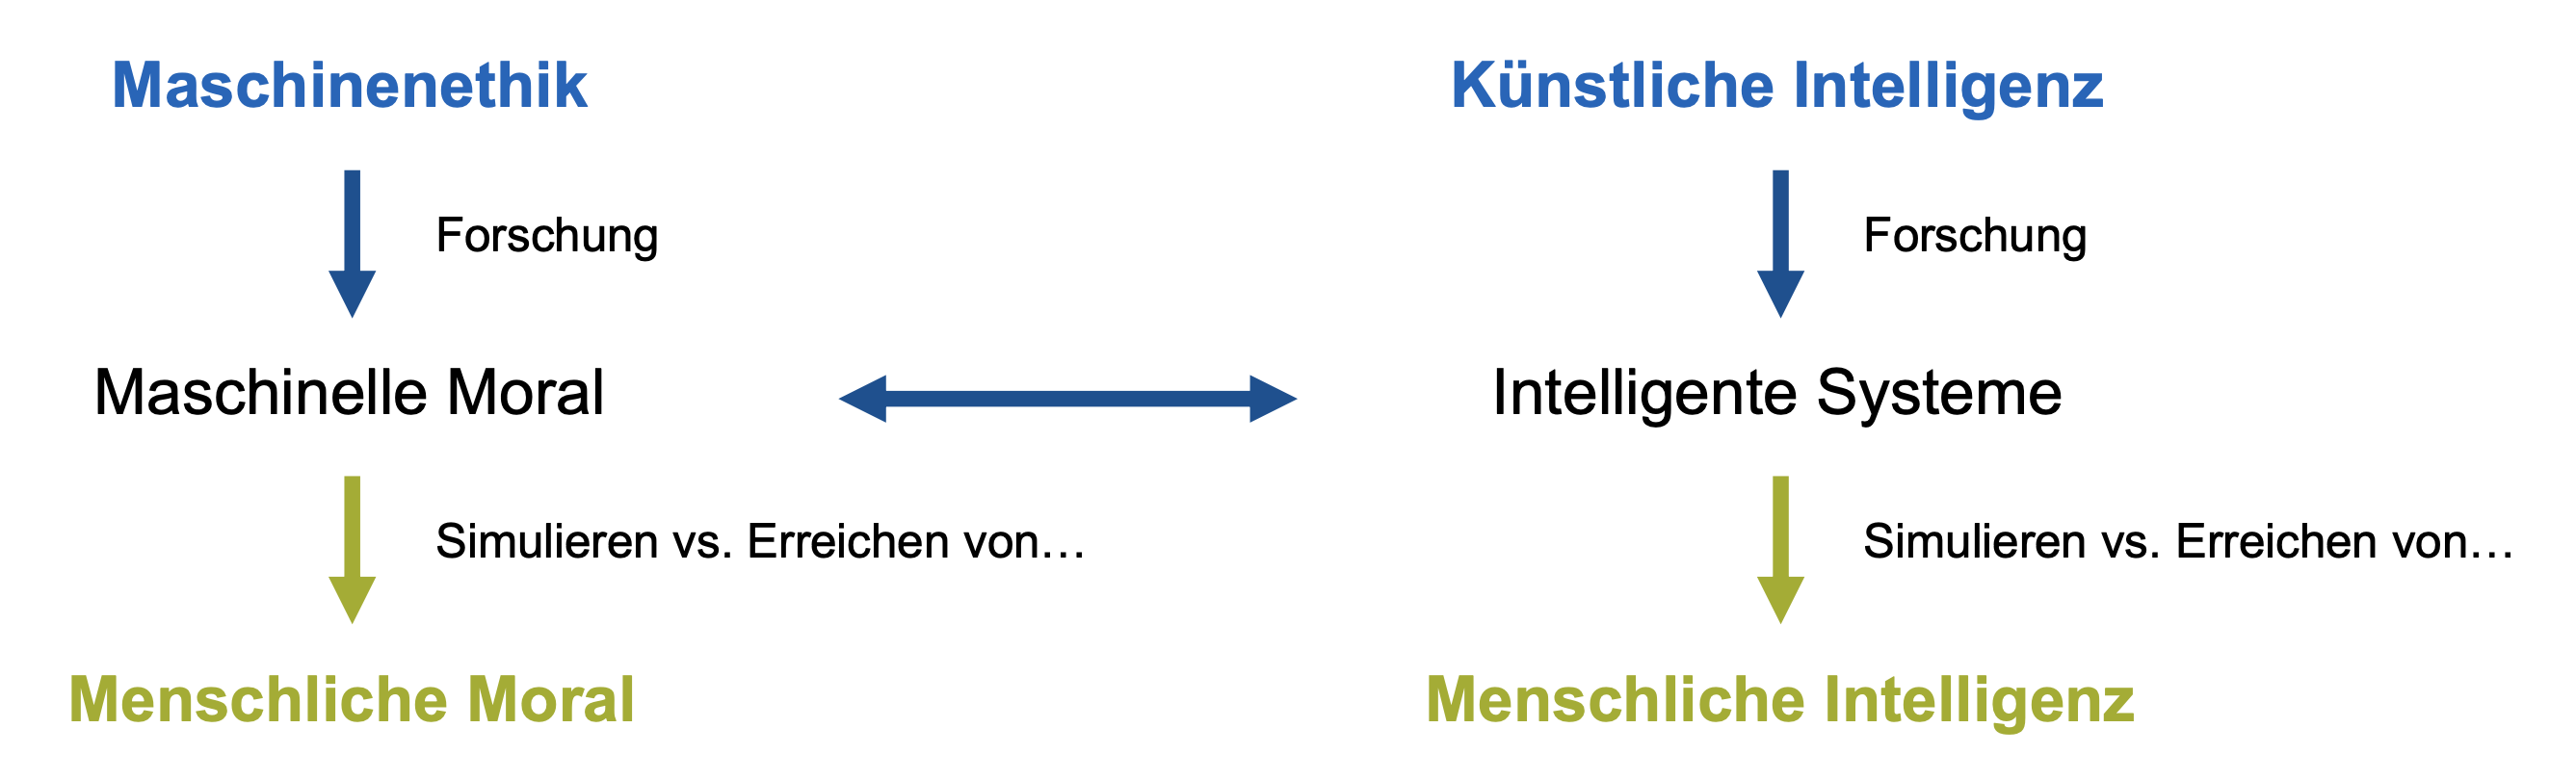
\includegraphics[width=\textwidth]{media/eth-int}
	\caption{Begriffliche Abgrenzung der maschinellen Moral und künstlichen Intelligenz~\cite[S. 17]{bendel-mascheth}.}
	\label{fig:moral-ethics}
\end{figure*}

Analog kann man die Differenzierung zwischen der schwachen und starken Eigenschaft von der Forschung zur künstlichen Intelligenz übernehmen.
Wir sprechen von schwacher maschineller Moral wie schwacher KI, wenn die entsprechende Eigenschaft simuliert oder in Teilen dem Vorbild nachgeahmt wird; erst die starke KI oder starke maschinelle Moral strebt danach, die Eigenschaft vollständig zu erreichen~\cite[S. 17]{bendel-mascheth}.
Die starke KI stellt hiermit also eine Art \emph{allgemeine} künstliche Intelligenz dar -- spätestens hier sind Überlegungen zur Moral in jedem Fall angebracht\footnote{Offen bleibt natürlich die Frage, ob die menschliche Moral in diesem Kontext das erstrebenswerte Ziel ist. Es kann ebenso Ziel sein, eine Art \glqq Moral\grqq{} zu erzeugen, die sich gänzlich von der des Menschen unterscheidet~\cite[S. 23]{bendel-mascheth}.}.

Abgegrenzt wird die Maschinenethik in der Regel von den mit ihr verwandten Bereichsethiken
\begin{itemize}
	\item der \textbf{digitalen Ethik}, die sich im Kern mit informationstechnologischen Systemen und den damit einhergehenden Überlegungen zu informationeller Autonomie auseinandersetzt, sowie
	\item der \textbf{Technikethik}, die sich allgemeiner gefasst mit technischen und wissenschaftlichen Entwicklungen beschäftigt und ebendiese mit ethischen Wertungen versieht.
\end{itemize}


\subsection{Kernfragen}
Die zentrale Idee der Maschinenethik ist also, die Maschine also als Subjekt und nicht nur als Objekt der Moral zu sehen -- sprich die Maschine im Sinne der Moral auf eine dem Menschen gleichgestellte Ebene zu heben.

Die Notwendigkeit dieser Überlegungen ergibt sich direkt aus der wachsenden Autonomie der Maschinen.
Trifft eine Maschine Entscheidungen, die ohne Zutun eines Menschen erfolgen, ist die Moral automatisch relevant.
Erst recht gilt dies, sofern dieser Maschine eine Entscheidungsgewalt über Leben und Tod zusteht.

Evident ist, dass für diese Art von extremer Entscheidungsfindung ein gewisses Verständnis des Kontext der Handlung nötig ist.
Konzepte wie Leben und Tod, Bewusstsein und Menschenwürde sind schwierig in imperative Programmzeilen zu encodieren -- genau das verlangen wir allerdings von moralisch entscheidenden Maschinen.

Die Disziplin stellt sich im Prinzip drei Kernfragen, die maßgeblich die Überlegungen charakterisieren (nach~\cite[S. 13ff.]{bendel-mascheth}):
\begin{enumerate}
	\item \textbf{Wie kommt die Moral in die Maschine?}

	Wie können wir es schaffen, das abstrakte Konzept einer \glqq Moral\grqq{} in ein für Maschinen verständliches Konzept zu verwandeln, inklusive aller Nuancen und Kontextüberlegungen die daraus folgen?
	
	\item \textbf{Wie viel Entscheidungsgewalt überlassen wir Maschinen?}

	Selbst, wenn wir von dem Vorhandensein einer maschinellen Moral ausgehen, bleibt die Frage offen, wie viel Macht wir dieser Maschine überlassen wollen.
	Ist es erstrebenswert, dass (vor allem in militärischen Anwendungsgebieten) die Maschinen vollständig autonom agieren können?
	
	\item \textbf{In welcher Form trägt die Maschine Verantwortung über ihr Handeln?}

	Unklar ist ebenfalls, inwieweit eine Maschine retrospektiv für eine getroffene Entscheidung oder durchgeführte Handlung zur Rechenschaft gezogen werden kann.
	Zur Illustration sei die folgende Frage gestellt: Bis wir zu vollständig selbstlernenden Maschinen gekommen sind, sind auch die fortschrittlichsten Computer in gewisser Weise an ihre Algorithmik oder ihre Trainingsdatenmenge gebunden; Kann man hier von Verantwortung sprechen?
\end{enumerate}


\subsection{Anwendungsgebiet autonomes Fahren}
Im Folgenden möchten wir uns auf das Anwendungsgebiet des autonomen Fahrens konzentrieren.
Dieses berührt alle drei der im vorigen Abschnitt aufgeführten Kernfragen, und ist nebenbei auch noch sehr Alltagsrelevant.
Wir haben als Gesellschaft viel Berührung mit den Überlegungen, die auf den kommenden Seiten folgen werden.
Gerade durch die Möglichkeiten einer zukünftig durch hochautomatisierte Fahrzeuge befahrene Innenstadt sprechen wir eben nicht von weit entfernten militärischen Operationen, sondern vom alltäglichen Straßenverkehr.

Die Motivation der technischen Entwicklung ist nach einem kurzen Blick in die Verkehrsunfallstatistik auf deutschen Straßen relativ klar erkenntlich.

Von den in 2018 ca. 2,5 Millionen polizeilich erfassten Verkehrsunfällen fußten ca. $88,4 \,\%$ maßgeblich auf dem Fehlverhalten der involvierten Fahrzeugführer (aus~\cite{kba-zulass},~\cite{destatis-grafik},~\cite{destatis-unfallaktuell}).
Das zeigt deutlich: der Faktor Mensch verschwindet vorerst nicht aus dem Straßenverkehr.
Immer und überall da, wo der Mensch beim Fahren konkrete Aktionen durchführt -- sei es Überholen, Einfädeln oder Abbiegen -- werden Fehler passieren.
Aus diesem Grund helfen seit geraumer Zeit diverse Assistenzsysteme im Fahrzeug mit.
Diese tragen maßgeblich zu der bis dato utopischen Vorstellung bei, dass wir mit deren Hilfe effizienter, eleganter und entspannter unterwegs sein werden.
Dazu müssen die Systeme ja nicht perfekt fahren -- sie müssen lediglich statistisch besser (und sicherer) fahren als wir.


\section{Technische Automatisierungsstufen nach der SAE}
\begin{figure*}
	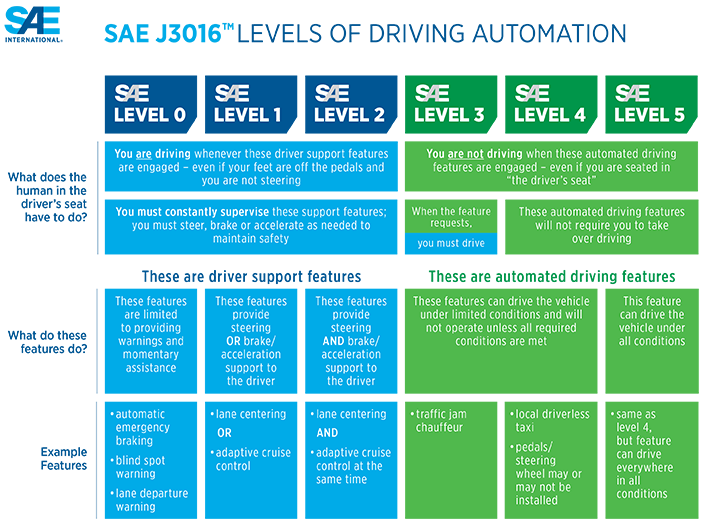
\includegraphics[width=\textwidth]{media/sae-levels-image}
	\caption{Die Automatisierungsstufen nach SAE-Standard J3016 (aus~\cite{sae-levels-image}).}
	\label{fig:sae-levels-img}
\end{figure*}

Zur Konkretisierung wird die technische Entwicklung an dieser Stelle in der Regel in sechs spezifische Automatisierungsstufen (auch \emph{Levels}) aufgeteilt.
Diese stellen aufsteigend das Fortschreiten von vollständig manuellem Fahren bis hin zur vollständigen Autonomie des Fahrzeugs dar.

Die Idee hinter einer derartigen Klassifizierung ist, dass hierdurch die Klärung der anfallenden rechtlichen und verantwortungstechnischen Fragen einfacher fällt.
Es lässt sich nun sehr einfach sagen, ab welchem Punkt die Maschine hier vorrangig die Verantwortung für ihr eigenes Handeln trägt -- eine Information, die in (straf-)rechtlichem Kontext durchaus wertvoll sein kann.

Im Folgenden möchten wir auf diese Automatisierungsstufen genauer eingehen (nach~\cite{sae-levels},~\cite{bast-levels}).

\subsection{Levels 0--2: menschlich gelenktes Fahren}
\begin{description}
	\item[Level 0.] Die überwiegende Mehrheit der Fahrzeuge auf deutschen Straßen ist mit der Automatisierungsstufe 0 unterwegs: als Selbstfahrer, bzw. \glqq Driver only\grqq{}.
	Hier übernimmt ganz klassisch der menschliche Fahrer alle Aspekte der Fahraufgabe\footnote{Was nicht bedeutet, dass keine technischen Features vorhanden sein können -- diese haben dann allerdings lediglich nur informierende oder isoliert eingreifende Wirkungen.}, und ist dementsprechend natürlich auch vollständig für sein eigenes Handeln verantwortlich.
	
	
	\item[Level 1.] Viele moderne Neuwagen bewegen sich nun mindestens auf dem Gebiet der Automatisierungsstufe 1, indem sie ihrem Fahrer bestimmte unterstützende und vor allem auf der Langstrecke der Ermüdung entgegenwirkende Assistenzsysteme anbieten.
	Dies kann beispielsweise ein adaptiver Tempomat sein, welcher im Kontrast zu einem regulären nichtadaptiven Tempomaten die eingestellte Geschwindigkeit unterschreitet, um den eingestellten Sicherheitsabstand zum vorausfahrenden Fahrzeug zu halten.
	Konkret geht es hierbei darum, dass die Technik jeweils ausschließlich entweder die Quer-, oder die Längssteuerung des Fahrzeugs übernehmen kann -- aber nicht beides gleichzeitig.
	Auch Spurwechselassistenten im Sinne von Totwinkelwarnern und Spurhalteassistenten mit der Möglichkeit zu einem korrigierenden, aber isolierten Lenkeingriff stellen hier also wertvolle Fahrhilfen dar.
	Eine Fahrhilfe ist allerdings genau das, was diese Systeme bieten: eine Hilfe beim Fahren für den eigentlichen Fahrer.
	Der Mensch fährt immer noch selbst und muss demnach bei der Verwendung der Systeme dauerhaft wachsam bleiben und jederzeit zur vollständigen und sofortigen Übernahme der Steuerung bereit sein.
	Somit liegt auch hier wie bei Level-0-Fahrzeugen die Verantwortung für Fahrhandlungen eindeutig beim Fahrzeugführer.
	
	
	\item[Level 2.] Als Beispiele für Fahrzeuge der Automatisierungsstufe 2 können sehr anschaulich die Fahrzeuge der Firma \emph{Tesla Motors} dienen.
	Diese sind mit dem \emph{Autopiloten} ausgestattet, der alle Level 2-Features anschaulich demonstriert~\cite{tesla-ap}:
	
	Diese Fahrzeuge sind gemäß der Spezifikation im SAE-Standard in der Lage, im Gegensatz zum Level 1 nun sowohl die Längs-, als auch die Querlenkung gleichzeitig zu übernehmen.
	Das System muss zwar vom Fahrer noch überwacht werden, kann allerdings in bestimmten Fahrsituationen (beispielsweise auf der Autobahn) das Fahrzeug eben autonom in der Spur halten und auch Gas und Bremse selbstständig bedienen~\cite[S. 1]{bast-levels}.
	Dies geschieht durch eine Mischung aus Kameradaten, lokaler Sensorik und GPS-basierten Kartendaten aus dem Navigationssystem.
	Darüber hinaus kann es bedingt durch die künstlich-intelligente Struktur der Programmierung während der Fahrt aus seinen eigenen Fehlern lernen und mit der Zeit bessere Fahrverhalten entwickeln.
	Begegnet das System allerdings einer Fahrsituation, mit der es nicht selbstständig umgehen kann, muss es die Steuerung sofort und ohne Verzögerung vollständig an den menschlichen Fahrer abgeben können.
	Somit steht auch hier der Fahrer bei allen Fahrsituationen oder im Falle eines Unfalls in der Verantwortung über die Aktionen des teilautonomen Fahrzeugs, und muss im Falle einer rechtswidrigen oder gefährlichen Situation unbedingt eingreifen.
\end{description}


\subsection{Levels 3--5: technisch gelenktes Fahren}
Aus ethischer Sicht interessant wird die Betrachtung allerdings erst richtig ab der nächsthöheren Automatisierungsstufe 3.
Ab hier bewegen wir uns nämlich in Gebieten, in denen das Fahrzeug zumindest streckenweise die Verantwortung für sein eigenes Handeln übernehmen muss.

\begin{description}
	\item[Level 3.] Ab hier übernimmt das autonome System nämlich in konkret abgesteckten Fahrsituationen komplett die Beobachtung der Umgebung sowie die angemessene Reaktion auf äußere Impulse.
\end{description}


\section{Unfallprävention und Unfallfolgenminimierung}
\subsection{Strategien in Systemgrenzbereichen}
\subsection{Reaktionen vs. aktive Entscheidungen}
\subsection{Deterministische Perspektiven}

\section{Typische Abwägungsszenarien}
\subsection{Die Parallele zum Trolley-Problem}
\subsection{Ethische Beispielargumentation}
\subsection{Versuch generalisierbarer Lösungsansätze}
\subsection{Die Moral Machine des MIT}

\section{Lösungsansätze der deutschen Ethikkommission}



\printbibliography

\end{document}
